\subsection{Visual Based Localization}

\label{sec:intro}

\begin{frame}{Content based image retrieval}

\end{frame}

\begin{frame}{Roadmap}

	We want to create an indirect method to localize a query within a set of \textbf{geolocalized} RGB-D images. The considered pipeline will be:
	
	\begin{figure}
		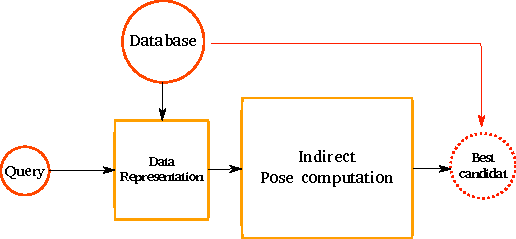
\includegraphics{vect/keys_comp_indirect.pdf}		
		\caption{Visual Based Localization (VBL) pipeline}
	\end{figure}		
		
\end{frame}

\begin{frame}{Data representation}
	We first focus our work on creating a robust data representation. Research on state of the art shown that CNN are the best choice~\cite{Arandjelovic2017}.
	
	\begin{block}{Encoder for data representation}
		\begin{figure}[c]
			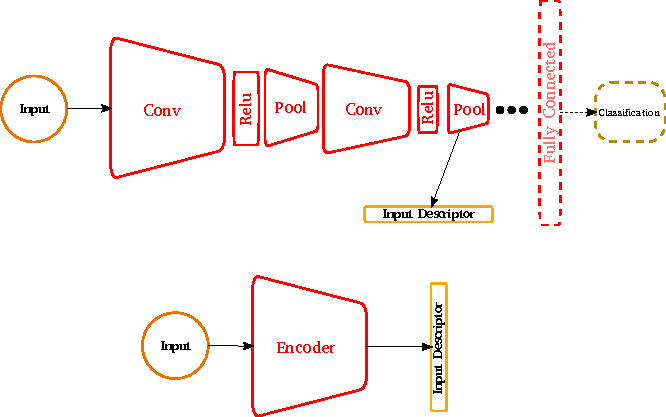
\includegraphics[width=0.75\linewidth]{vect/encodeur.pdf}					
		\end{figure}
	\end{block}
	
\end{frame}

